
This section elaborates on the concepts presented in the introduction.

\section{Approximate Computing}
Approximate computing, transprecision computing~\citep{malossi2018transprecision}, mixed- and reduced precision computing~\citep{cherubin2019taffo} are related concepts that unite under the goal of trying to improve computer resource usage or computation speed through approximation of some kind. It is not a novel concept, for instance the development of stochastic computing, which is a form of computation based on controlled randomness, began in the late 60s for the same reasons as today: a decrease in improvements within hardware development~\citep{sym16121701}. Stochastic computing fell out of favor when transistors became smaller and more reliable, but has in recent times become a topic of interest like the rest of approximate computing. 

Approximate computing does not require any special tooling to implement, and isn't dependent on specialized hardware either. Some examples of this include memoization~\citep{mittal2016survey}, a technique that involves caching results of expensive computations;  loop perforation~\citep{li2018sculptor}, which is removing some iterations of certain types of loops; or utilizing types that take up less bits in memory, for instance replacing 64 bit numbers with 32 bit numbers~\citep{cherubin2019taffo, tagliavini2018flexfloat, floatsmith_paper}. These methods can all be performed by the programmer without the use of tools. Doing all this manually however requires the programmer to instrument the program to verify that the output is within the required bounds of precision, and whether any of the steps taken makes the program behave unexpectedly. For this reason there have been created several tools aimed at research on the utility of approximate computing that encompass both the execution of the code and verification of the results. 

%figures of approximate computing techniques?
\subsection{Approximate Computing Through Reducing the Amount of Bits (Precision Scaling)}
\label{section:approximate_computing_through_reducing_bits}

Of all the techniques listed, only in the bit width modification category were there any software available for download or development. The most relevant of these are \floatsmith{}~\citep{floatsmith_paper} and \taffo{}~\citep{cherubin2019taffo}. In the papers describing them they are capable of reducing the precision of a program written using floating point variables through the usage of C/C++ annotations (that can normally be safely ignored by a compiler), and propagates changes throughout the program without having to annotate all variables in the program.

\emph{FloatSmith} aims to achieve mixed precision programs that vary the size of the floating point numbers used throughout, selecting from the IEEE 754-2008 Standard for Floating-Point Arithmetic~\citep{ieee754} for single- (32 bit), double- (64 bit), quad- (128 bit) and half-precision (16-bit) floating point numbers. Floating point numbers are very common today because of their versatility for programmers, as they can cover a larger range of values than a regular binary integer representation given the same amount of bits.

For the programmer, in theory it is not even necessary to annotate the code. The annotations are used by a tool in the \floatsmith{} toolchain, ADAPT. It is used to narrow the search space of potential optimization candidate variables.

Figure~\ref{fig:float_bit_representation} shows a 8-bit representation of a floating point number using the same principles as the IEEE standard, but with arbitrarily selected bit widths of the different sections of the bits. 

\begin{figure}[h]
    \centering
    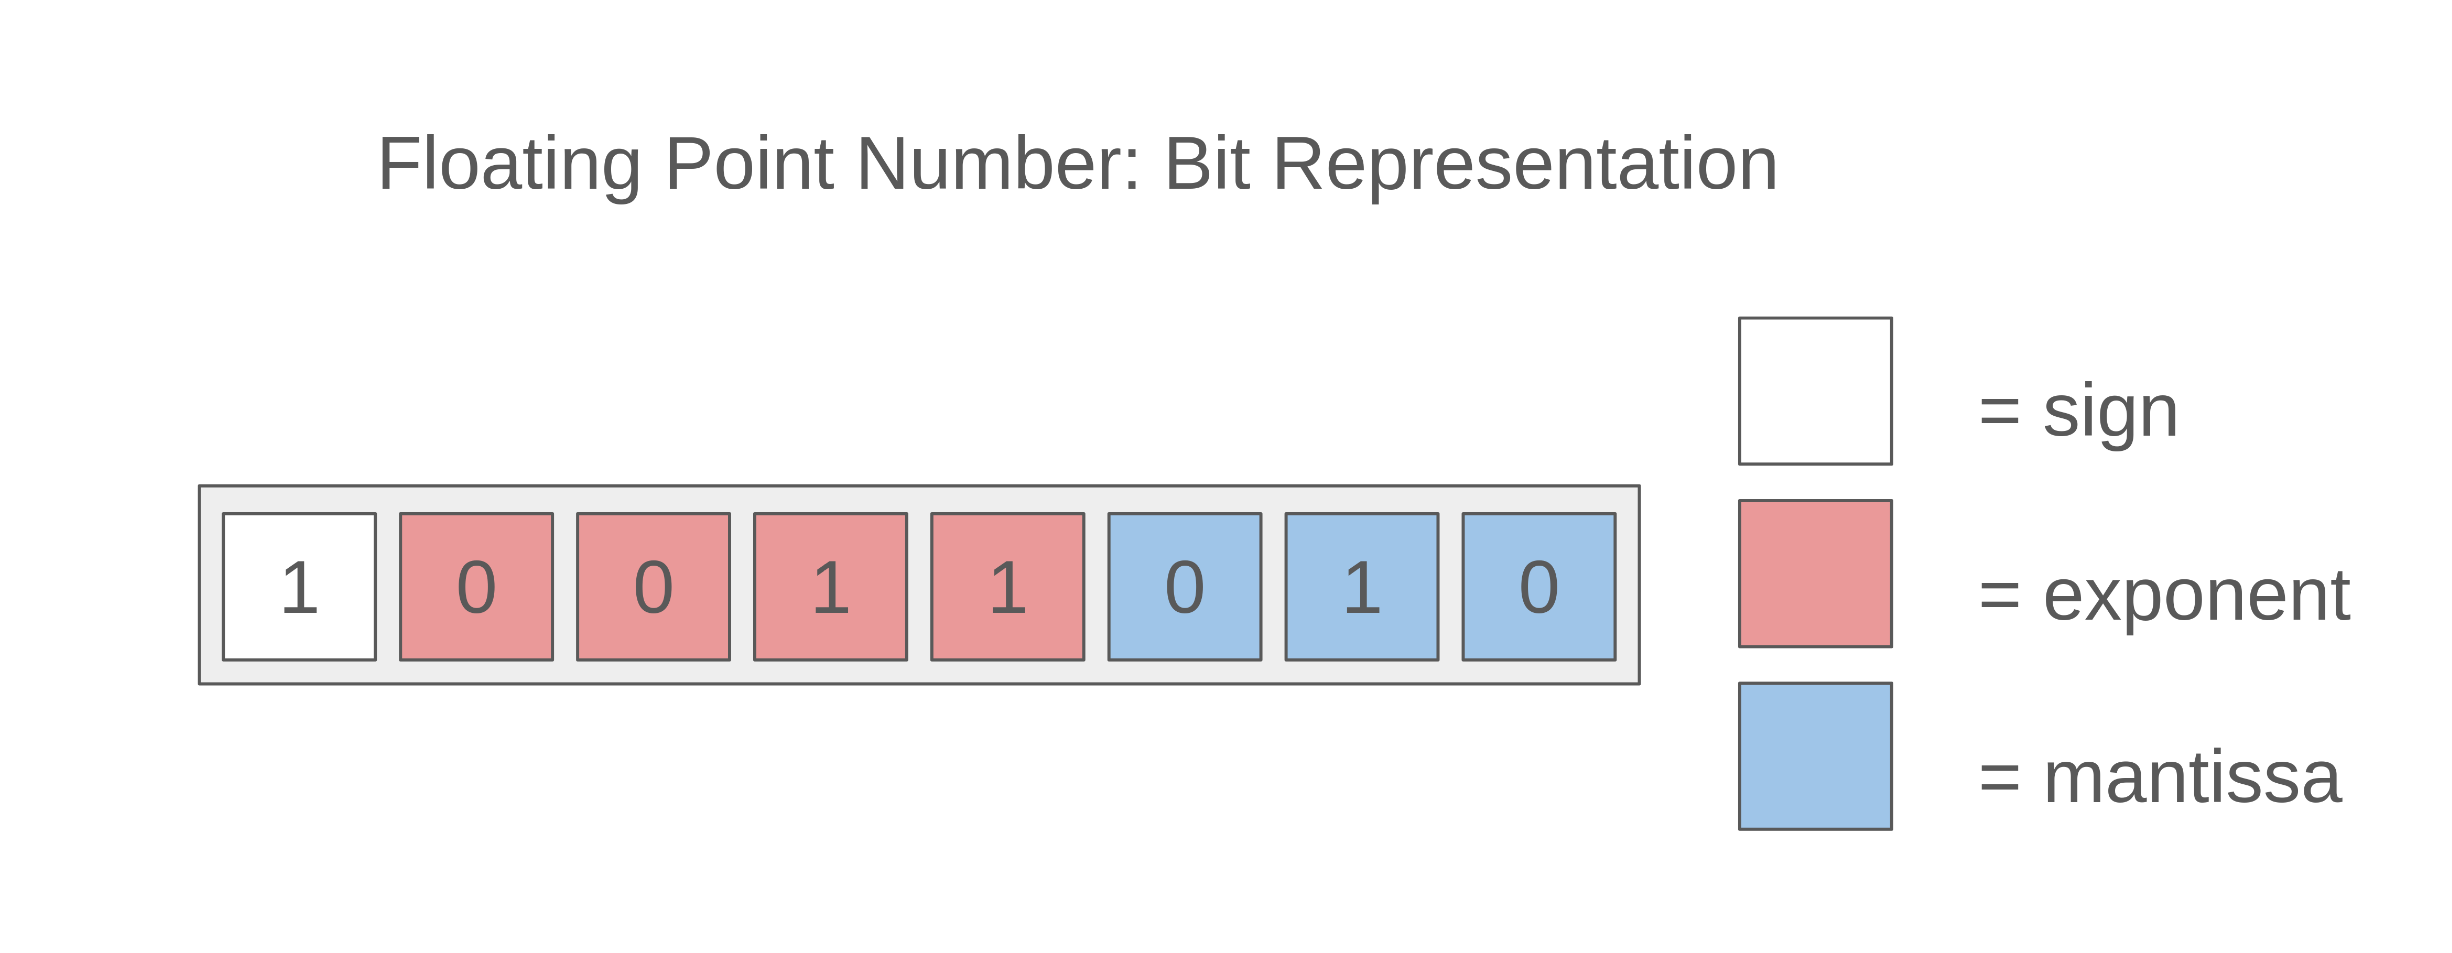
\includegraphics[width=0.75\linewidth]{Images/float_bit_representation.png}
    \caption{Simplified floating point representation of a number, in this case the number -0.15625}
    \label{fig:float_bit_representation}
\end{figure}

Equation~\ref{eq:float} shows the equation that corresponds to the decimal value of a floating point number stored in this format. The IEEE 754-2008 Standard has predefined bit widths for the exponent and mantissa sections, this example disregards these and operates with the sizes in figure~\ref{fig:float_bit_representation}: One sign bit, four exponent bits and three mantissa bits.

\begin{equation}\label{eq:float}
    (-1)^{bit_7} * 2^{(exponent) - 7} * mantissa \, value
\end{equation}

The sign bit decides whether the number is positive or not. Using the values in figure~\ref{fig:float_bit_representation}, the equation for the sign bit value is shown in equation~\ref{eq:float1}.

\begin{equation} \label{eq:float1}
    (-1)^{1} = -1
\end{equation}

The exponent part of the floating point number decides the exponent part of the equation. The IEEE standard defines the exponent part of the number using an implicit negative offset, such that if all exponent bits except the most significant bit (bit at index 6) in figure~\ref{fig:float_bit_representation}) are set to 1, the exponent is 0. For the arbitrary floating point format shown in figure~\ref{fig:float_bit_representation}, the offset becomes $2^4 - 1$, which is 7. Plugging in the values from figure ~\ref{fig:float_bit_representation} gives us the value shown in equation~\ref{eq:float2}:
\begin{equation} \label{eq:float2}
    2^{4-7} = 2^{-3}
\end{equation}

The final part of the floating point number, the mantissa, also known as the fraction or the significand, is usually the largest part (with respect to the amount of bits  it takes up in a binary representation, i.e., the bit width) of a floating point number.
The value of the mantissa is calculated as with an integer represented in binary, only starting at bit index 2 the bit value is $(bit\,value)*2^{-1}$, the value at bit index 1 is $(bit\,value)*2^{-2}$, and so on. Additionally, an implicit value of the integer 1 is added to the mantissa. Plugging the values from figure~\ref{fig:float_bit_representation} into the mantissa part of the of the equation gives the value shown in equation~\ref{eq:float3}:

\begin{equation}\label{eq:float3}
   1 + 0*2^{-1} + 1*2^{-2} + 0*2^{-3} = 1.25
\end{equation}

Plugging the values from equations~\ref{eq:float1},~\ref{eq:float2} and~\ref{eq:float3} into equation~\ref{eq:float} gives us:
\begin{equation}\label{eq:float4}
-1 * 2^{-3} * 1.25 = -0.15625
\end{equation}

The IEEE standard describes special cases for when all bits in the exponent are either 1 or 0 to deal with special situations, but this is not important for a basic understanding of how the bit representation works.


CPUs that support floating point numbers have dedicated hardware for floating point math. Performing calculations with smaller bit width floating point numbers do not yield any significant gains, so using FloatSmith on a program will only yield a better result energy-wise if the CPU is required to fetch and store fewer bits from memory, thereby widening the storage bottleneck in processing~\citep{floatsmith_paper}. 

\taffo{} also performs approximate computing through changing the precision of variables, but instead of switching between different bit width floating point numbers, \taffo{} transforms floating point numbers to fixed point representation, using programmer hints through annotations about the range of values that the variables can contain. Listing~\ref{listing:taffo_annotation} shows an example annotation of a variable taken from the seidel-2d benchmark that is used later on in the thesis.


\begin{lstlisting}
int i __attribute__((annotate("scalar(range(-" PB_XSTR(N) ", " PB_XSTR(N) ") final)")));
\end{lstlisting}

The annotation is made using the \_\_attribute\_\_ keyword, the contents of which can be ignored if the compiler does not support it. The annotation is connected to the variable i in this case. the "scalar" keyword is used on homogeneous types such as floats or ints, or collections such as arrays or matrices with only one type. The "scalar" keyword contains the minimum and max value that the variable can contain, and finally the "final" keyword
The description of the annotation syntax is contained within the \taffo{} repository in the folder doc/AnnotationSyntax.md. 

Figure~\ref{fig:fixed_point_representation} shows an arbitrary number and its negative counterpart in fixed point binary representation. Fixed point is the "default" representation of numbers, and is how integers are stored in memory.

\begin{figure}
    \centering
    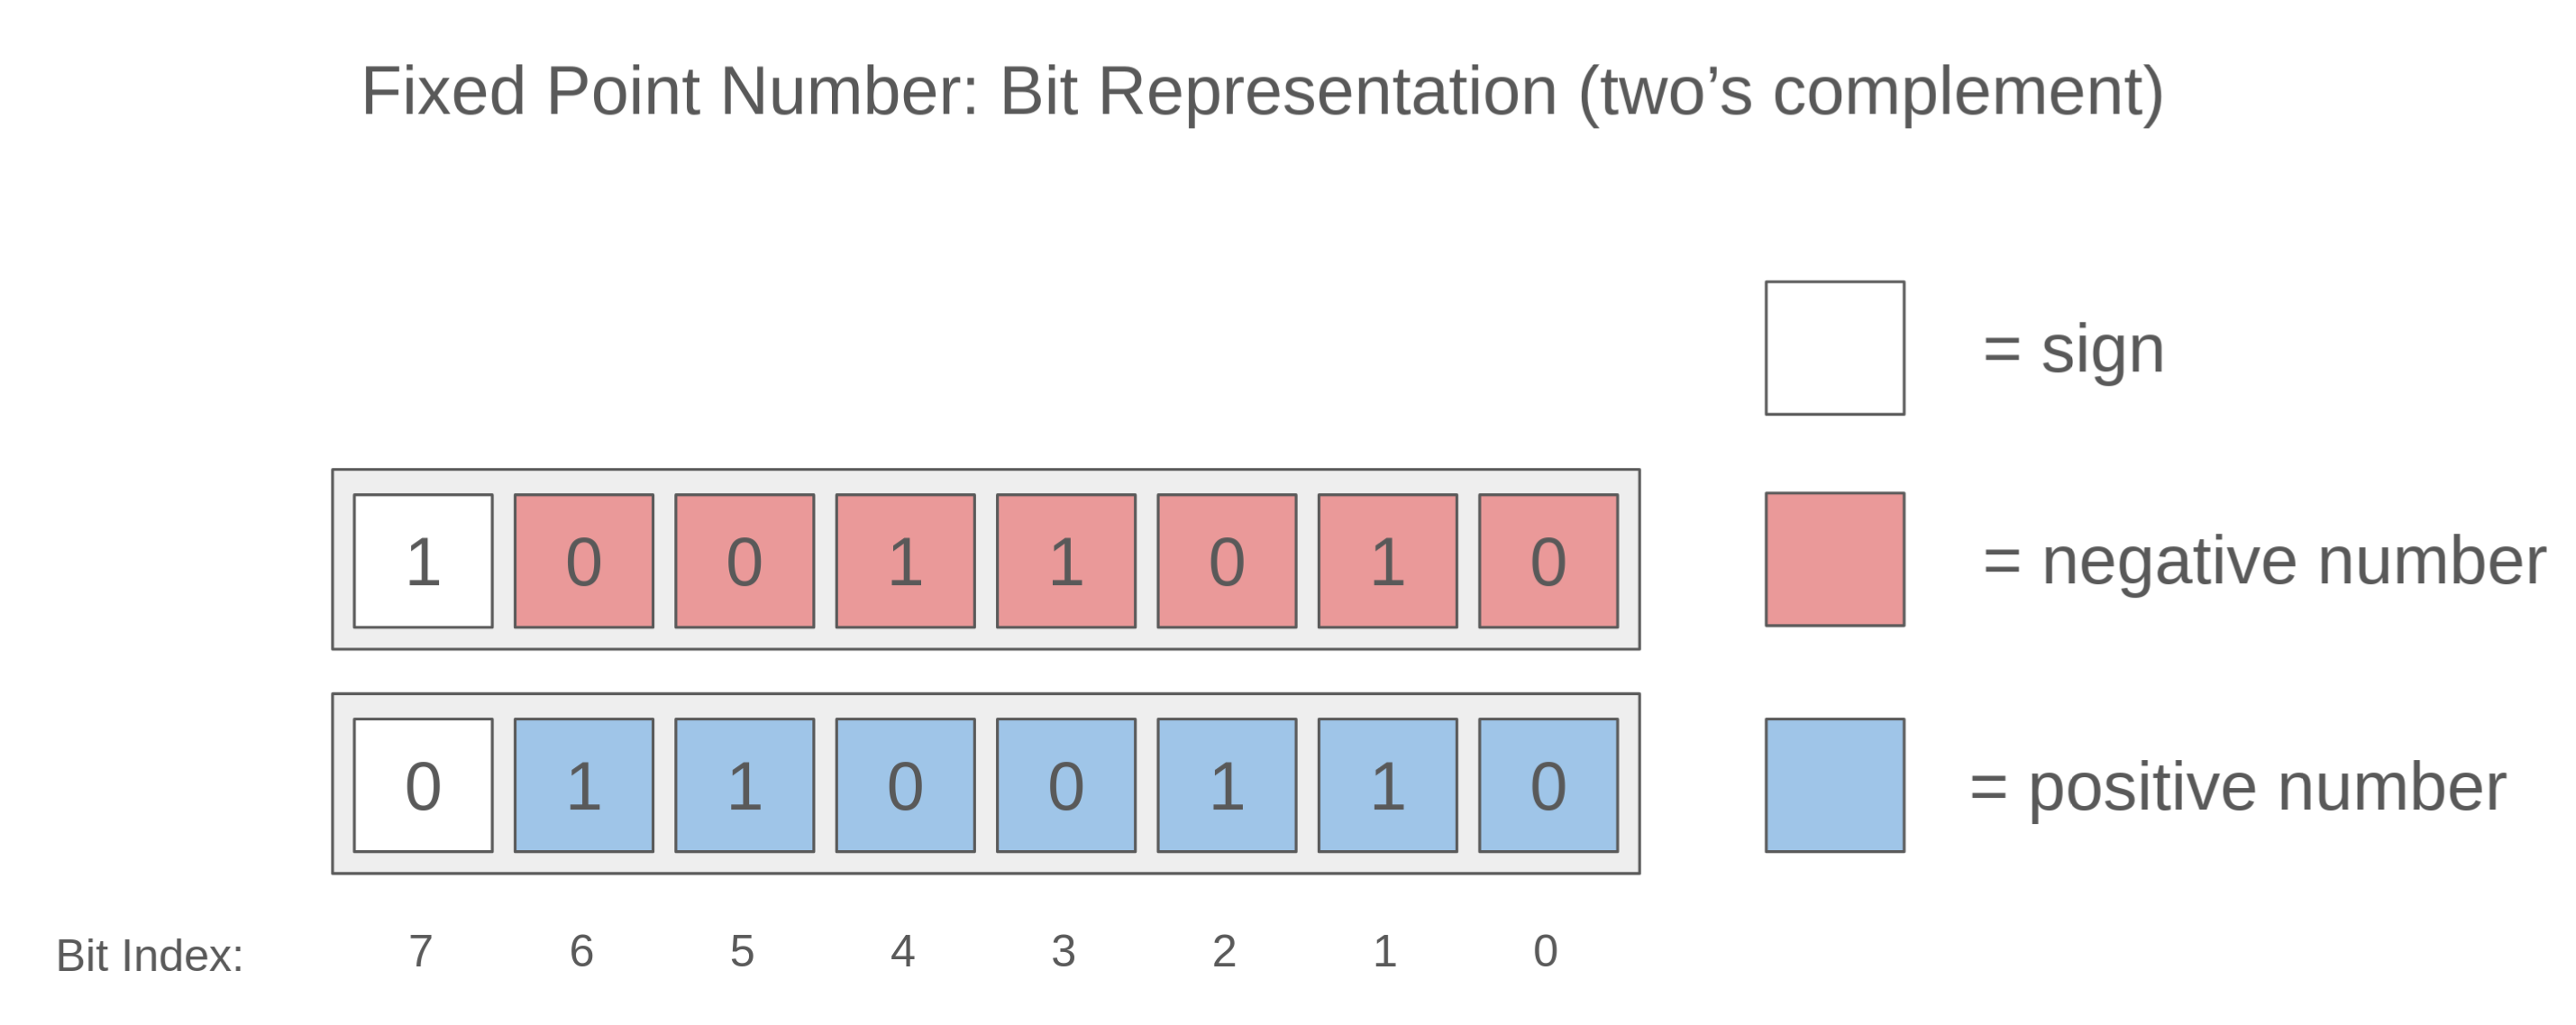
\includegraphics[width=0.75\linewidth]{Images/fixed_point_bit_representation.png}
    \caption{Fixed point representation of a number in binary using the two's complement method.}
    \label{fig:fixed_point_representation}
\end{figure}

Fixed point decimal numbers are represented by allocating a fixed amount of bits for the fractional part, and a fixed number of bits for the integer part, and in the case that it is a signed number the most significant bit is the sign bit. This is implicit and not visible in how a processor treats the numbers, which means that the processor can use the same hardware for operating on fixed point decimal numbers as regular integers. 
% This is often faster than performing operations on floating point numbers. 
It becomes the programmer's job to manage which bits are in front of and behind the decimal point within the code itself (in C, and other languages that don't directly support fixed point decimal math). 

% \todo{should I include description of how to perform math with fixed point numbers in code?}

Therefore, depending on the program, the numerical values for the bit representations in figure~\ref{fig:fixed_point_representation} could be 102 for the positive and -102 for the negative if we do not use a scaling factor, or if we decide that the three lower bits should be the fractional part of the number, to get our output number we must perform a right shift three places for the integer part of the number: 1100, which gives us the integer -4. Shifting a binary to the right is the same as dividing by two to the power of however many positions were shifted, so in this case that number is $2^3 = 8$. This is the scaling factor. The rightmost part of the fixed point number is divided by this scaling factor to get the part of the number behind the decimal point. 110 in binary is the same as 6 in integer representation which gives us $6/8 = 0.75$, making the number represented -4.75. The processor does not see the decimal point in a fixed point number, only an integer, and the math operations stay the same. The programmer however needs to supply the CPU with integers that are scaled to account for the decimal point. For instance, to add or subtract the integer 1 to the number, first we need to scale the number according to the scaling factor. In this case, this means shifting the number to the left three places, making the value we are adding/subtracting look like the value 8 to the CPU. Multiplication however requires no change in the numbers supplied.  For more details, see~\citet{yates2009fixed}.

\taffo{} therefore depends on users of the program to annotate a variable that is to be converted to a fixed point type with the range of values it can have, which is used to decide how many bits is required to represent the number accurately enough as a fixed point number. 


% There are other papers detailing other methods of approximate computing. Sadly, though they are described vividly in the papers, efforts to get a hold of these approximate computing tools proved fruitless. In the following sections, some of the papers detailing these elusive tools are described.


Besides precision scaling there are other common software techniques that have been integrated in tools for augmenting a program, the most prominent of these are loop perforation and memoization. These tools would also have been subject to study, had they not been impossible to get a hold of, even through contacting the authors. 


\subsection{Approximate Computing through Loop Perforation}

Loop perforation, described by \citet{li2018sculptor} and \citet{baek2010green}, works by skipping iterations in loops that iteratively get closer to an accurate number. The Gauss-Seidel benchmark included in the polybench CPU benchmark~\citep{polybench} is an example of a loop that may be optimized with loop perforation. Loop perforation would not work on just any loop, such as a loop reading in lines of data from a file, as this could cause data corruption and program crashes.

\subsection{Approximate Computing through Memoization}

Memoization consists of mapping the inputs of expensive functions to their outputs, and avoiding to re-run the function for the same input, thereby saving energy. This is described more in depth by \citet{mittal2016survey}.


\section{Reliability through Fault Tolerance}
\label{section:Reliability_thorugh_fault_tolerance}

Reliability is a concept that concerns itself with whether a system provides correct service or not. A system in this context could be a software component such as a software library, or an entire computer system coupled with software such as an ATM machine. Correct and incorrect service is not necessarily a rigid concept for all types of systems. In the case of an ATM machine, correct service requires cash withdrawals to match the amount withdrawn from an account exactly for all clients, while a computer vision face detection library that detects a face in 90 out of 100 images that contain faces may be considered correct service.

\citet{avizienis2004basic} provides a stricter definition the concept of reliability, as well as dividing reliability into multiple related concepts. Of these, the most relevant to this thesis is the definitions of fault tolerance, service failure, errors, and faults.  

Fault tolerance is a prerequisite of reliability. Fault tolerance is defined as the continued delivery of correct service in spite of faults present in the system. A fault is an artifact that may result in an error, and an error is an internal state of a part of the system that does not correspond with the defined correct states. An error does not necessarily end up affecting the external state (the output of the system), but the moment that an error does affect the external state to an incorrect state, this constitutes a service failure.

\citet{avizienis2004basic} divide faults into two categories: developmental faults, or operational faults. Faults are divided into one of the two depending on when they occur: developmental faults occur during the development of the system, and operational faults occur while the system is providing service. A software bug would be a developmental fault, and a bit flip caused by ionizing radiation would constitute an operational fault.



Code quality is important to achieve fault tolerant code, and should be evaluated alongside the operational fault tolerance of a software tool. While the operational aspect is certainly important, i.e., how the code responds to faults that occur during operation, a project's code quality will affect the amount of faults that are created during the developmental phase, which carry equivalent risk of causing service failures during operation. 

% There are multiple papers on the investigation of fault tolerance through hardware fault injection, see section~\ref{section:Verifying_fault_tolerance} for a more thorough overview. 

\subsection{Quantifying Fault Tolerance}
\label{section:Verifying_fault_tolerance}

Different applications have different fault tolerance requirements; a satellite orbiting the earth would necessarily have much higher requirements with respect to operational fault tolerance due to ionizing radiation than a run-of-the-mill home computer. Developmental fault tolerance requirements in software governing an industrial complex will also be stricter than the software governing a smart home system. 

Given these requirements, one way of verifying or quantifying the fault tolerance of a system is through fault injection.

Fault injection is a controlled insertion of faults into a system, with the goal of observing the resulting state of the system with these additional faults inserted. Fault injection can be performed through ionizing radiation, heat or applying local voltages to the hardware. Fault tolerance experiments such as these are performed mostly to evaluate hardware that will be subjected to harsh conditions. 
Fault injection can also be performed in software. For instance,~\citet{venkatagiri2019gem5} describe a software system that flips individual bits in the program, and simulates the running of these programs to find all bits in a program that are conducive to silent data corruptions (failures that don't stop the service delivery, but delivers an incorrect service).  G-SWFIT is a methodology of injecting software faults that would otherwise fall outside of what a programmer would normally catch during testing~\citep{natella2012fault}.

There are frameworks for injecting both operational and developmental faults allowing users to gauge fault tolerance in a way that otherwise would be difficult: Given a lack of the resources required to perform hardware fault injection as \citet{arlat1993fault} describe, software alternatives like Xception~\citep{carreira1998xception} that allows the user to emulate hardware bit flips in a program, or the Gem5-approxilyzer described by \citet{venkatagiri2019gem5} that allows users to simulate how single bit flips propagate instruction by instruction through a processor, can provide accurate alternatives.

Fault injection can and should be performed during the developmental phase of both software and hardware systems. 
\citet{natella2012fault} describe an approach to software fault injection using fault statistics for a category of software to infer potential fault locations that would not be caught by regression testing. 
Evaluating tests by injecting faults that should be caught by those tests is a strategy commonly referred to as mutation testing, the goal of which is to create code "mutants" (versions of your code that contain an injected error), and then "killing" the mutants with the test suite, i.e.,  the test suite catches unexpected behavior through tests failing.

When access to the source code is limited, faults can still be injected in software through the entry points provided in the code. In computer security circles one such approach is known as fuzzing~\citep{miller1990empirical}, and is useful both as a fault tolerance testing tool of non-open source binaries, and as a tool for simulating adversarial activity in the input interfaces of a tool.

\section{LLVM bytecode}
The fault injection performed in this thesis is performed in LLVM bytecode.
LLVM bytecode is an assembly-like programming language used as an intermediate representation within the LLVM suite of compiler tools. LLVM is not an acronym, though in the early stages of the project it used to stand for Low Level Virtual Machine. These tools are mostly made for performing code transformations, and these transformations are made on LLVM bytecode. The LLVM tools relevant to this thesis is the core optimizer known as opt, and Clang for compiling C/C++~\citep{LLVM_homepage}.  %explain llvm 

\taffo{} is comprised of LLVM optimization passes. These optimization passes are performed on LLVM bytecode, and clang is used to compile source code (with custom made annotations denoting the range of the variables) to LLVM bytecode. %how taffo figures in this

